

\chapter{Predictive digital twins at scale for piles}
\label{DT}

This chapter develops a mathematical and computational foundation for digital twins of piles.

While the value proposition of digital twins has become widely appreciated, the technology itself remains in a custom production phase.



\section{State space model}



\section{Probabilistic graphical model: Control theory }




\section{Partially observable Markov decision process}

As shown in \cref{fig: POMDP}, based on Markov Chain, with introducing Rewards and Actions, it can form the basis of Partially observed Markov decision process.
\begin{figure}[H]
    \centering
    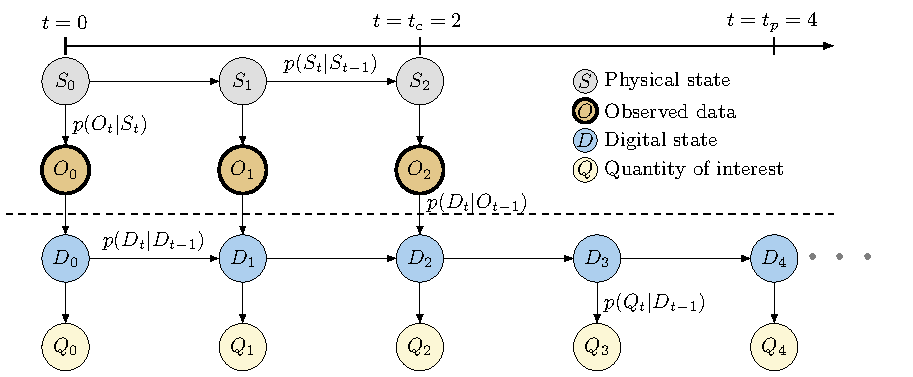
\includegraphics[width = 140mm]{Figures/figure-POMDP.pdf}
    \caption{Digital twin}
    \label{fig: POMDP}
\end{figure}
Generally, Digital Twin can be divided into two main parts, including (1) calibration and assimilation (2) Prediction, as shown in \cref{eq: DA_predict}  and \cref{eq: DA_assimilation}.
\begin{equation}
\begin{aligned}
& p(D_{0},...,D_{t_{c}},Q_{0},...,Q_{t_{c}},R_{0},...,R_{t_{c}}|o_{0},...,o_{t_{c}},u_{0},...,u_{t_{c}}) \\
& = \prod_{t=0}^{t_{c}}[\phi_{t}^{update}\phi_{t}^{QoI}\phi_{t}^{evaluation}] \label{eq: DA_predict}
\end{aligned}
\end{equation}
\begin{equation}
\begin{aligned}
    & p(D_{0},...,D_{t_{p}},Q_{0},...,Q_{t_{p}},R_{0},...,R_{t_{p}},U_{t_{c}+1},...,U_{t_{p}}|o_{0},...,o_{t_{c}},u_{0},...,u_{t_{c}}) \\
    & \propto \prod_{t=0}^{t_{p}}[\phi_{t}^{dynamics}\phi_{t}^{QoI}\phi_{t}^{evaluation}] \prod_{t=0}^{t_{c}}\phi_{t}^{assimilation} \prod_{t=t_{c}+1}^{t_{p}}\phi_{t}^{control} \label{eq: DA_assimilation}
\end{aligned}
\end{equation}
\section{Computational model-ICFEP}

\section{Planning and prediction via digital twin}